\chapter{Introduction}
\label{ch:introduction}

\todo[Thesis format]

Reproducibility is a cornerstone of scientific research. The ability to reproduce a study in order to verify or build on the results is an important part of a thriving scientific community. Reproducibility is contingent on access to the original data and methodology. In 2015, Radford et al. published an article introducing deep convolutional generative adversarial networks (DC-GAN), a class of convolutional networks that works with unsupervised learning. The original Torch implementation of DC-GAN is available on GitHub\footnote{https://github.com/soumith/dcgan.torch} and was created by Soumith Chintala\footnote{https://github.com/soumith}, one of the co-authors of the original publication. The original DC-GAN implementation was modified to be used with TensorFlow, an alternative deep learning framework, and hosted on GitHub\footnote{https://github.com/carpedm20/dcgan-tensorflow} with links to the original publication and original code as shown in Figure \ref{fig:dcgan-tensorflow}. In 2018, Tabassi et al. published an article that used DC-GAN in a workflow to create a dataset to test the accuracy of software product. Tabassi et al. referenced the original publication and included a link to the TensorFlow implementation, the exact implementation they leveraged in their workflow. This is one example of researchers building on the software products created by previous research. If the original code had not been available in a public repository, Tabassi et al. would not have been able to implement DC-GAN in their workflow without significant time replicating what had already been created by the previous researchers. 

\begin{figure}
    \centering
    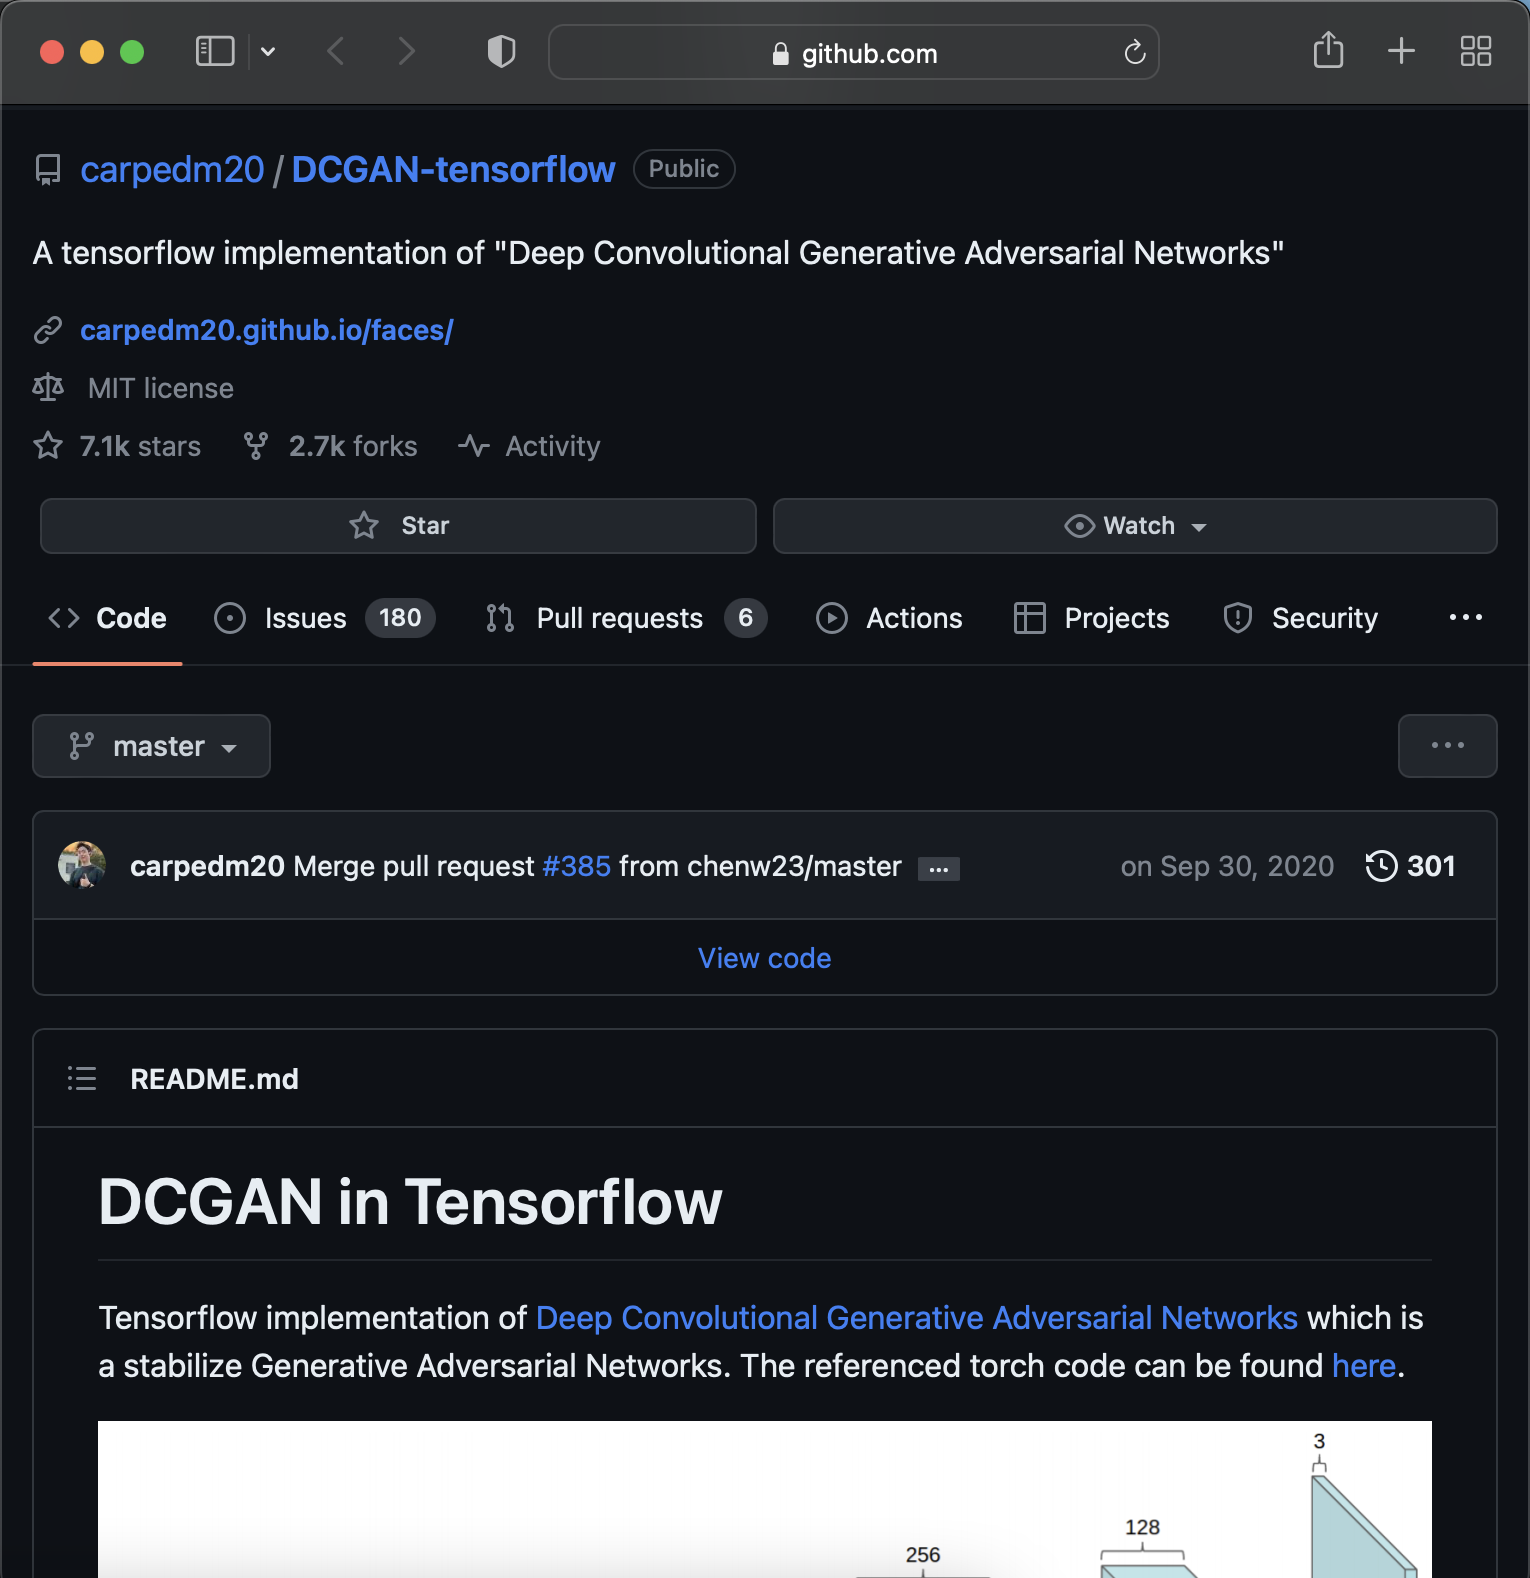
\includegraphics[width=\linewidth]{dcgan-tensorflow.png}
    \caption{The TensorFlow implementation of the original Torch DC-GAN implementation includes links to the original publication and original code hosted in GitHub.}
    \label{fig:dcgan-tensorflow}
\end{figure}


Not all researchers are as fortunate. Lane et al. published an archive pre-print that references a GitHub repository\footnote{https://github.com/tjlane/odin} as the implementation of the framework proposed in the article (Figure \ref{fig:arxiv-odin}). However, the repository is no longer available on the live Web as shown in Figure \ref{fig:odin-404}. Fortunately, both Internet Archive and Software Heritage, two archives that will be further explained in Chapter 2, archived the repository while it was still alive. Internet Archive captured the repository three times from August 19, 2017 to November 17, 2020 with the latest capture showing that the repository was no longer publicly available. Software Heritage captured the repository 11 times from August 4, 2015 to February 27, 2020. If Internet Archive and Software Heritage had not captured the repository, future researchers would not have been able to access the implementation of the methodology detailed in the article. 

\begin{figure}
    \centering
    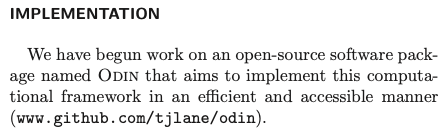
\includegraphics[width=\linewidth]{arxiv-odin.png}
    \caption{The authors indicate that the exact implementation of the methodology detailed in the article can be found at the indicated URL.}
    \label{fig:arxiv-odin}
\end{figure}

\begin{figure}
    \centering
    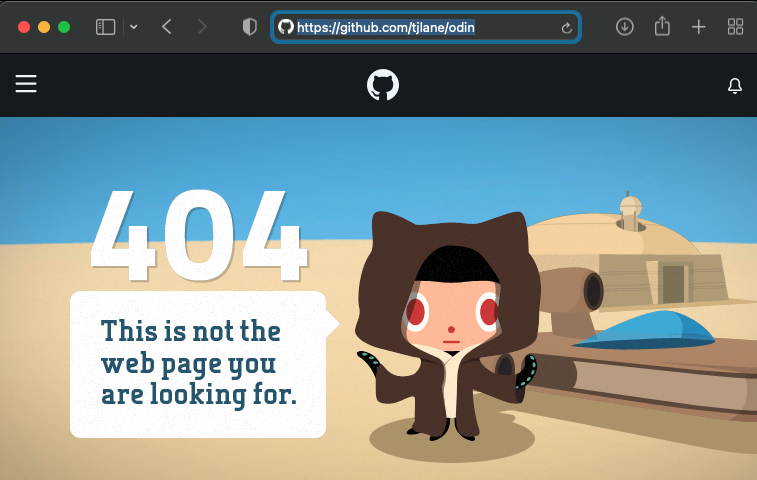
\includegraphics[width=\linewidth]{odin-404.png}
    \caption{The repository at \url{github.com/tjlane/odin} is no longer publicly available on the live Web.}
    \label{fig:odin-404}
\end{figure}

Scientific researchers like Tabassi et al. and Lane et al. are increasingly including URLs to source code repositories to supplement the methodology they detail within their publications. Additionally, open access initiatives and mandates are increasing the availability of open access data and software. However, software availability that satisfies an open access requirement is different than software preservation. If a repository ceases to be available on the live Web, a lack of software preservation has the potential to nullify the advantages gained by open access data and software requirements. Additionally, the need for software preservation spans farther than the computer science discipline. Software development as a research output is increasingly prevalent in research across disciplines from biology to physics to economics. Software products contain the exact methodology used in the study and allow the study to be reproduced both by the original researchers and future researchers.

To address the problems faced by researchers, we investigated the prevalence of URIs to Git Hosting Platforms (GHPs) like GitHub, GitLab, SourceForge, and Bitbucket in scholarly publications. We also investigated the preservation of these scholarly code products in the archives. This work will present the results of our studies in the form of four research questions:

RQ1: How often do authors include GHP URIs in scholarly articles?

RQ2: For the GHP URIs identified in scholarly articles, what is the prevalence of these GHP URIs (a) on the live Web, (b) in Software Heritage, and (c) in Web archives?

RQ3: Outside of GHPs, what OADS URIs are scholars including in their publications?

RQ4: Does GitHub popularity affect the likelihood of a repository being archived? 
